\section{Atribuição de valor a imagens de refeições}

\subsection{Arquitetura do sistema}


\subsection{Modelos de NN considerados e sua avaliação}

Keras é uma API de redes neurais de alto nível, escrita em Python e capaz de rodar em cima do TensorFlow, CNTK ou Theano que pode rodar na CPU ou GPU.

Aplicações Keras são modelos de deep learning que são disponibilizados juntamente com pesos pré-treinados. Esses modelos podem ser usados para previsão, extração de recursos e ajuste fino.

Os modelos disponíveis para classificação de imagens com pesos treinados no ImageNet são:

\begin{itemize}
    \item Xception
    \item VGG16
    \item VGG19
    \item ResNet50
    \item InceptionV3
    \item InceptionResNetV2
    \item MobileNet
    \item DenseNet
    \item NASNet
    \item MobileNetV2
\end{itemize}

Todas essas arquiteturas são compatíveis com todos os backends (TensorFlow, Theano e CNTK).

Os modelos utilizados nesse trabalho foram o MobileNetV2, DenseNet121 e o NASNetMobile.

\subsubsection{MobileNetV2}
Em 2017, um grupo de pesquisadores do Google publicou um artigo que apresentava uma arquitetura de rede neural otimizada para dispositivos móveis. Essa arquitetura chamada de MobileNets são modelos pequenos, com baixa latência e baixo consumo de energia parametrizados para atender às restrições de recursos de vários casos de uso. Eles podem ser construídos para classificação, detecção, incorporação e segmentação, semelhante a como outros modelos populares de grande escala, como o Inception, são usados. Os MobileNets podem ser executados de forma eficiente em dispositivos móveis com o TensorFlow Mobile.

%https://ai.googleblog.com/2017/06/mobilenets-open-source-models-for.html

%https://towardsdatascience.com/mobilenetv2-inverted-residuals-and-linear-bottlenecks-8a4362f4ffd5

A capacidade de executar redes profundas em dispositivos móveis pessoais melhora a experiência do usuário, oferecendo acesso a qualquer hora, em qualquer lugar, com benefícios adicionais para segurança, privacidade e consumo de energia. À medida que novos aplicativos surgem, permitindo que os usuários interajam com o mundo real em tempo real, o mesmo acontece com a necessidade de redes neurais cada vez mais eficientes. Por isso, a Google apresentou uma nova versão dessa arquitetura esse ano, o MobileNetV2.


O MobileNetV2 é uma melhoria significativa em relação ao MobileNetV1 e impulsiona o estado da arte para reconhecimento visual móvel, incluindo classificação, detecção de objetos e segmentação semântica. O MobileNetV2 baseia-se nas ideias do MobileNetV1, porém, a V2 introduz dois novos recursos à arquitetura: Resíduos Invertidos e Gargalos Lineares.

Em comparação com a primeira versão, no geral, os modelos do MobileNetV2 são mais rápidos com a mesma precisão em todo o espectro de latência. Em particular, os novos modelos usam duas vezes menos operações, precisam de 30\% menos parâmetros e são cerca de 30-40\% mais rápidos em um telefone do Google Pixel do que os modelos do MobileNetV1, tudo isso com maior precisão.

%https://ai.googleblog.com/2018/04/mobilenetv2-next-generation-of-on.html

\begin{figure}[!ht]
\centering 
\caption{O MobileNetV2 melhora a velocidade (latência reduzida) e aumenta a precisão do ImageNet Top 1}
\label{fig:mobilenetv1vsv2}
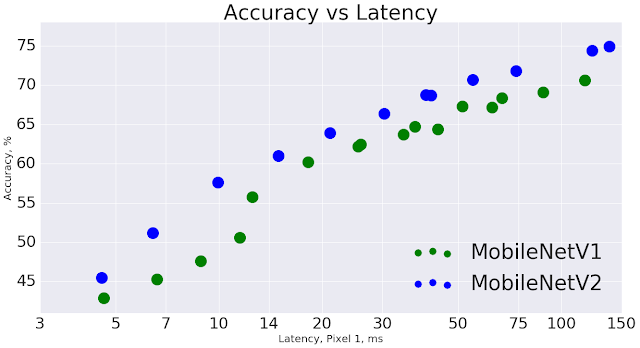
\includegraphics[width=0.9\textwidth]{imgs/mobilenetv1vsv2.png}
\end{figure}


\subsubsection{DenseNet121}

À medida que as CNNs se tornam cada vez mais profundas, surge um novo problema de pesquisa: conforme as informações sobre a entrada ou gradiente passam por várias camadas, elas podem desaparecer antes de chegar ao fim da rede.

%https://arxiv.org/pdf/1608.06993.pdf

Redes Convolucionais Densamente Conectadas (DenseNets) simplificam o padrão de conectividade entre camadas introduzidas em outras arquiteturas. Os autores resolvem o problema garantindo o fluxo máximo de informações (e gradientes). Para fazer isso, eles simplesmente conectam cada camada diretamente entre si. Em vez de extrair poder de representação de arquiteturas extremamente profundas ou amplas, as DenseNets exploram o potencial da rede por meio do reuso de recursos. As DenseNets requerem menos parâmetros que um CNN tradicional equivalente, já que não há necessidade de aprender mapas de recursos redundantes.

DenseNets, em contraste com ResNets, nunca combinam recursos por meio do somatório antes de serem passados para uma camada. Em vez disso, combinam recursos concatenando-os.
Assim, a camada l tem l entradas, consistindo nos mapas de características de todos os blocos convolucionais precedentes. Seus próprios mapas de características são passados para todas as camadas subsequentes de L-l. Isso introduz as conexões L (L + 1) 2 em uma rede de camada L, em vez de apenas L, como nas arquiteturas tradicionais. Devido ao seu denso padrão de conectividade, a abordagem foi chamada de Dense Convolutional Network (DenseNet).

\begin{figure}[!ht]
\centering 
\caption{Um bloco denso de 5 camadas com uma taxa de crescimento de k = 4. Cada camada usa todos os mapas de recursos anteriores como entrada.}
\label{fig:densenet}
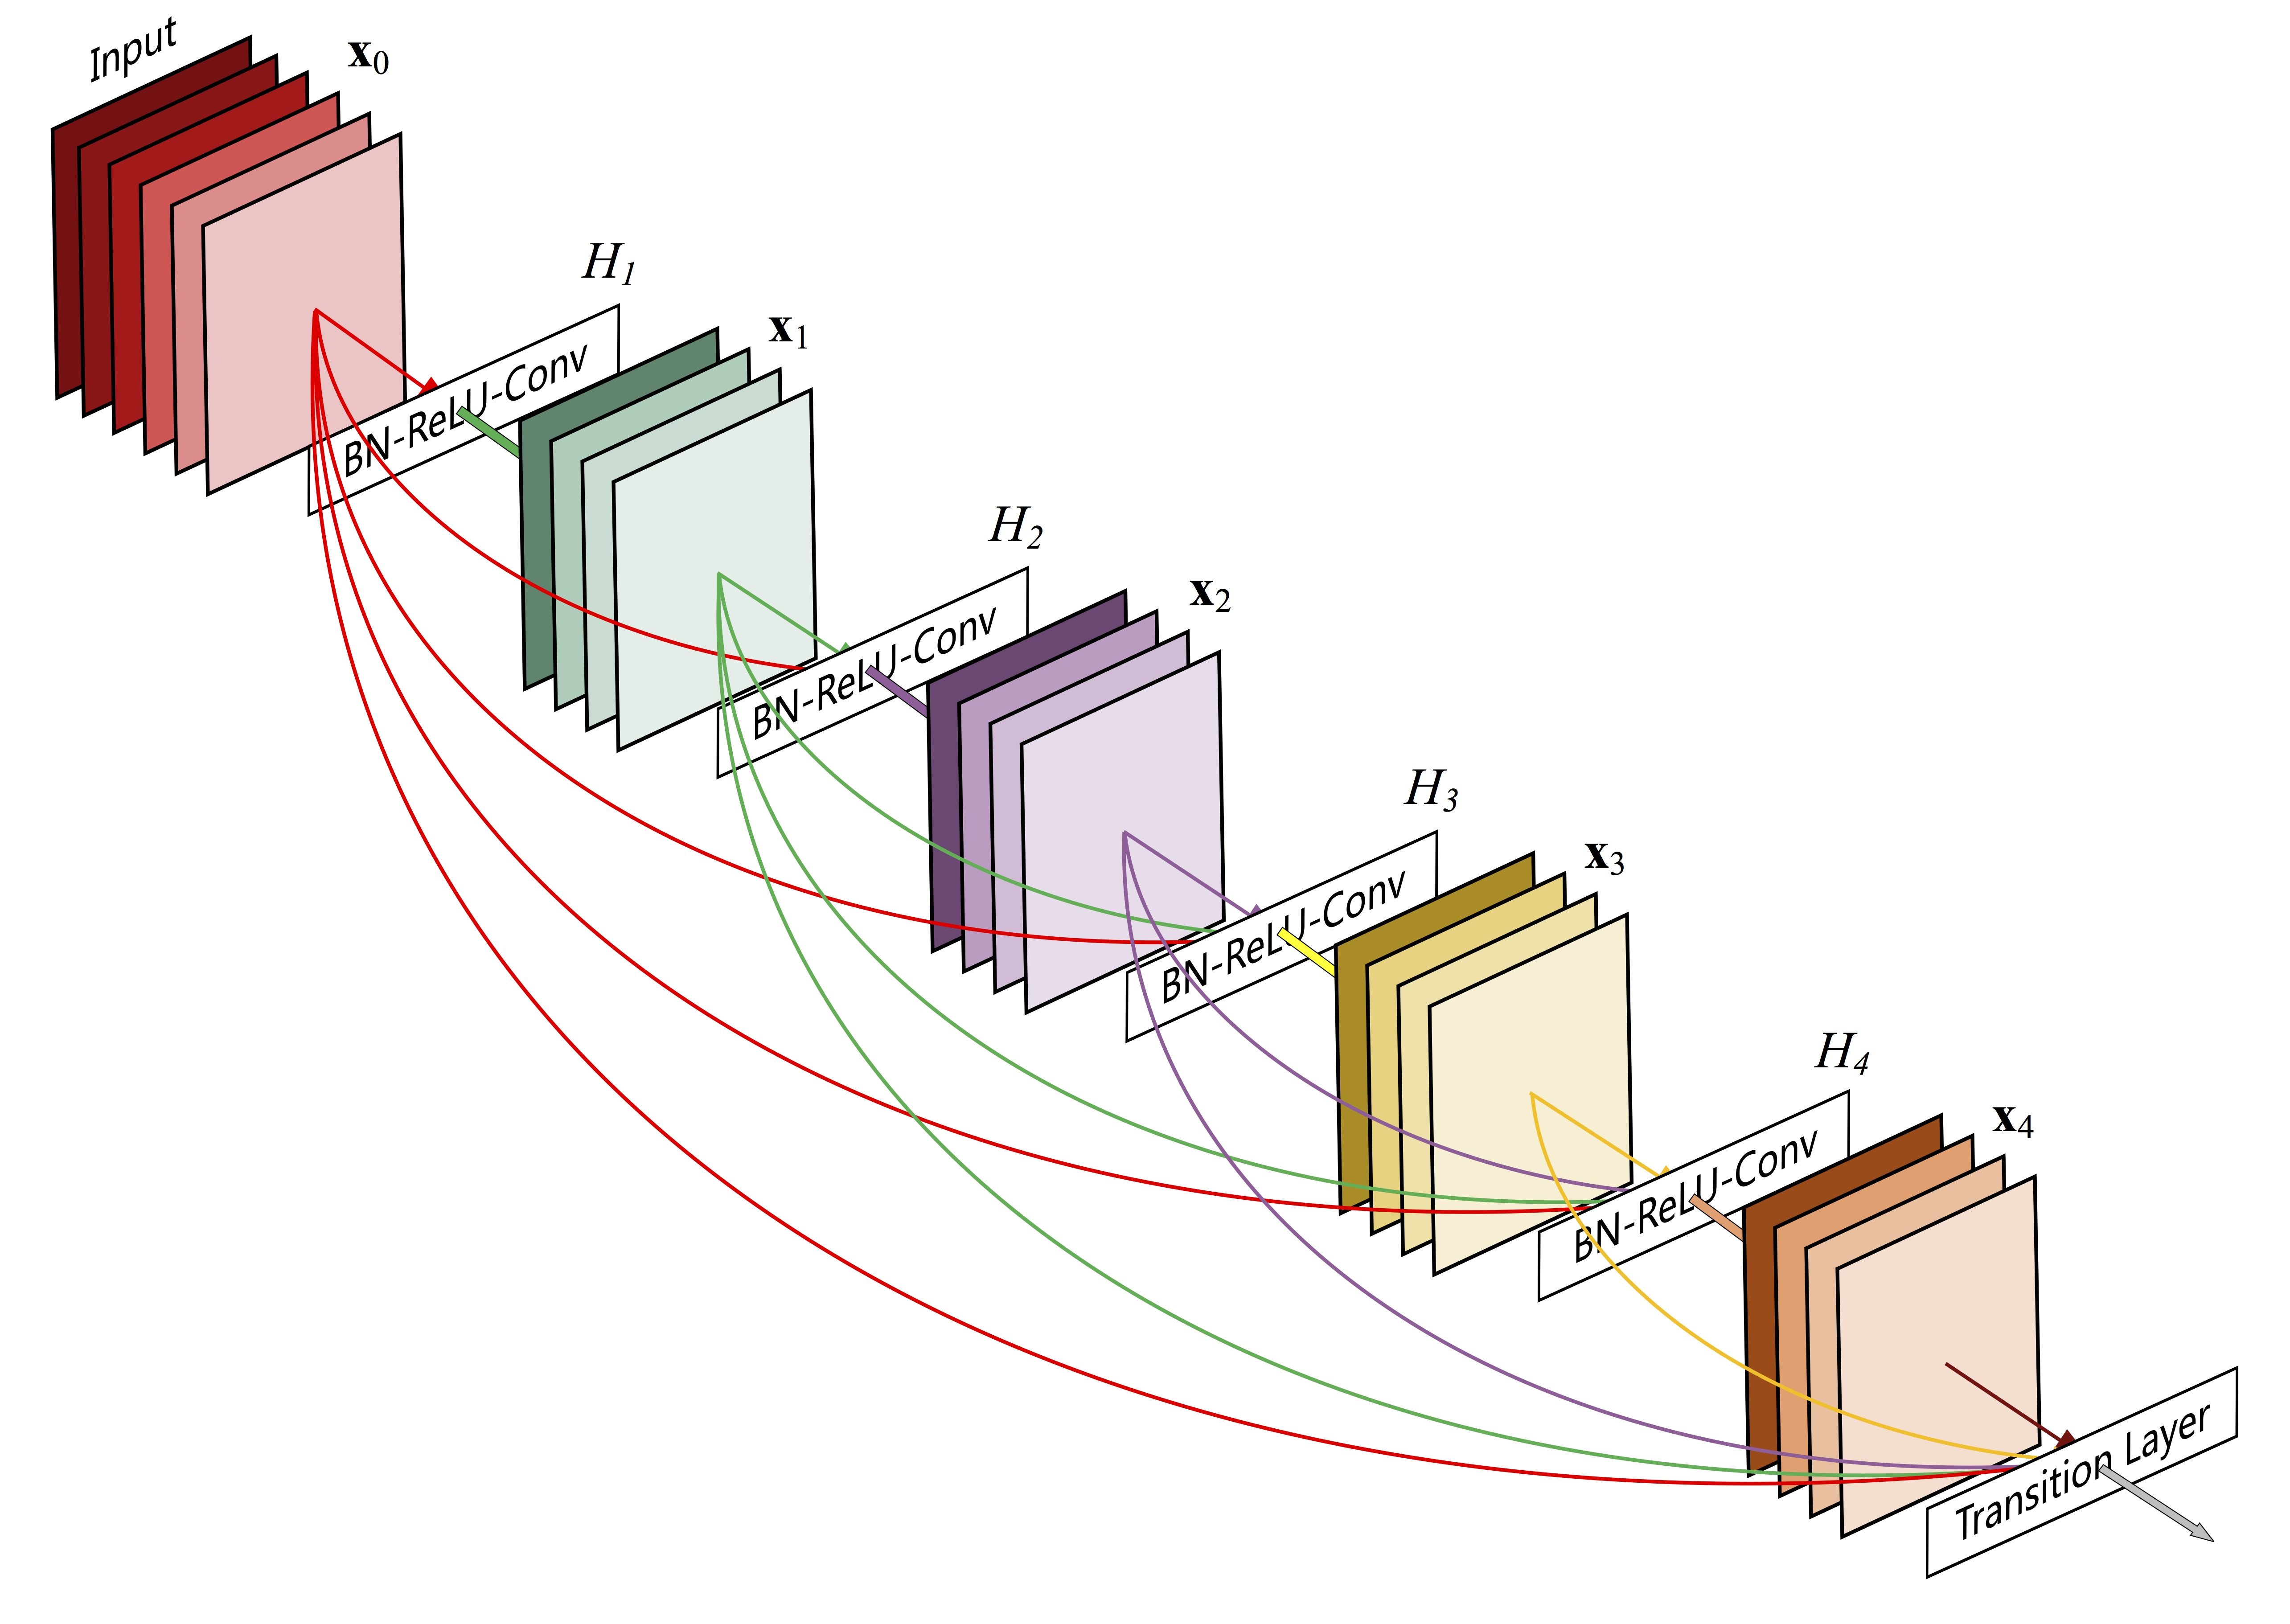
\includegraphics[width=0.9\textwidth]{imgs/densenets.jpg}
\end{figure}

\subsubsection{NASNetMobile}

%https://towardsdatascience.com/everything-you-need-to-know-about-automl-and-neural-architecture-search-8db1863682bf